\label{chap:p2-mckee}
\section*{Preamble}
Paper II employs the system developed in Chapter~\ref{chap:p1-system} to determine the time to maximum vasoconstriction of subcutaneously injected epinephrine. Previous work was performed with porcine models using laser Doppler flowmetry and estimated the time interval to be 7 to 10 minutes in length.\cite{Larrabee1987} This work was performed in 1987 and there had been no further investigation to confirm this result prior to this work. In this paper, lidocaine was injected into volunteers upper arms with and without epinephrine to induce reddening or blanching respectively, and DRS measurements were performed every 1 to 2 minutes over the course of 2 hours. Since work was still being performed on a spectrally-constrained model (see Chapter~\ref{chap:p3-model}), the measurements were analyzed with the commonly cited Dawson erythema index.\cite{Dawson1980}

The protocol used during this investigation was developed primarily by the author of this thesis (further known as ``the author'') with contributions by Dr. D. McKee (the first author of the paper). In addition, the majority of the material required for the Research Ethics Board application was prepared by the author. Injection of the lidocaine (and epinephrine) was performed by Dr. McKee while all subsequent measurements were performed by the author with assistance from Dr. McKee. The program for converting the measurements into corrected Dawson erythema indices was written and executed by the author while the error analysis and the interpretation of the time course results was undertaken by Dr. McKee. The manuscript was prepared primarily by Dr. McKee under the supervision of Drs. D. Lalonde and A. Thoma. The author and Dr. J. Hayward did not contribute major changes to the manuscript. The manuscript has been altered from its original form to match the style of this thesis.

\section*{Contents}

\begin{center}

\textbf{Optimal Time Delay between Epinephrine Injection and Incision to Minimize Bleeding}

Daniel E. McKee, Donald H. Lalonde, Achilleas Thoma, Diana L. Glennie, and Joseph E. Hayward

\textit{Division of Plastic and Reconstructive Surgery, Department of Surgery, and the Department of Medical Physics and Applied Radiation Sciences, McMaster University, 1280 Main Street West, Hamilton, Ontario, L8S 1A8}

\textit{AND}

\textit{Saint John Regional Hospital, Dalhousie University}

\end{center}

\noindent Journal of Plastic and Reconstructive Surgery \textbf{131}(4), 811-814 (April 2013).

\noindent \url{http://dx.doi.org/10.1097/PRS.0b013e3182818ced}

\section*{Abstract}

\noindent \textbf{Background:} The time until maximal cutaneous vasoconstriction after injection of lidocaine with epinephrine is often given in textbooks and multiple choice examinations as 7 to 10 minutes. However, in our experience, there is significantly less cutaneous bleeding if one waits considerably longer than 7 to 10 minutes after injection of local anesthesia with epinephrine for most procedures on human skin.

\noindent \textbf{Methods:} This was a prospective, randomized, triple-blind study where 12 volunteers were injected simultaneously in each arm with either 1\% lidocaine with epinephrine (study group) or 1\% plain lidocaine (control group), after which the relative hemoglobin concentration of the underlying skin and soft tissues was measured over time using spectroscopy.

\noindent \textbf{Results:} In the epinephrine group, the mean time at which the lowest cutaneous hemoglobin level was obtained was 25.9 minutes (95 percent CI, 25.9 $\pm$ 5.1 minutes). This was significantly longer than the historical literature values of 7 to 10 minutes for maximum vasoconstriction after injection. Mean hemoglobin index values at every time measurement after postinjection minute 1 were significantly different between the study group and the control group, with use of a two-tailed paired t test (p < 0.01).

\noindent \textbf{Conclusions:} If optimal visualization is desired, the ideal time for the surgeon to begin the incision should be 25 minutes after injection of local anesthetic with epinephrine. It takes considerably longer than 7 to 10 minutes for a new local equilibrium to be obtained in relation to hemoglobin quantity.

\noindent \textbf{CLINICAL QUESTION/LEVEL OF EVIDENCE:} Therapeutic, I.

\noindent \textcopyright 2013 American Society of Plastic Surgeons

\section{Introduction}
Epinephrine is routinely used with local anesthetic in surgical procedures to provide hemostasis, where visualization of underlying intricate anatomy is important. The time until maximal cutaneous vasoconstriction after injection of lidocaine with epinephrine is often listed in textbooks\cite{Knize2007,Kryger2007} and multiple-choice examinations as 7 to 10 minutes. This value originated from a 1987 study using a laser Doppler flowmeter on pig skin after injection of 1\% lidocaine with epinephrine at several concentrations, including 1:100,000.\cite{Larrabee1987} In our clinical experience, there is significantly less cutaneous bleeding if one waits considerably longer than 7 to 10 minutes after injection of local anesthesia with epinephrine for most procedures on human skin.

The purpose of this study was to see how long it really takes to obtain the lowest cutaneous hemoglobin concentration after lidocaine with epinephrine injection in the human arm. In this prospective, randomized, triple-blind study, volunteers were injected simultaneously in each arm with either 1\% lidocaine (plain) or 1\% lidocaine with epinephrine. The underlying skin and soft-tissue perfusion changes were monitored with diffuse reflectance spectroscopy to estimate relative hemoglobin concentration changes over time. The time until the lowest concentration of hemoglobin was obtained for each volunteer injected with lidocaine with epinephrine.

\section{Patients and Methods}
This study was given final full approval on December 8, 2011, from the Research Ethics Board affiliated with Hamilton Health Sciences and McMaster University (project no. 11-543) and all volunteers gave informed written consent. Between March and May of 2012, 12 volunteer university students with ages ranging from 21 to 31 years, and a male-to-female ratio of 50:50, received two injections within 1 minute of each other just under the dermis on the lateral arm over the deltoid insertion. One person was responsible for injecting all volunteers: 5 cc of 1\% lidocaine with 1:100,000 epinephrine (0.01 mg/ml) in one arm and 5 cc of 1\% lidocaine (plain) in the other arm (AstraZeneca Canada, Inc., Mississauga, Ontario, Canada). By opaque envelope, volunteers were assigned randomly with details of arm allocation so that they had a 50:50 chance of receiving the epinephrine injection in either their left or right arm. The study was triple-blinded: neither the volunteer, the person injecting the local anesthetic, nor the spectroscopy technician knew which arm was injected with which solution. With regard to volunteer skin type, 11 volunteers were white and one was of eastern Asian heritage.

Spectroscopy measurements were taken every minute from each arm for 5 minutes before injections and for 30 minutes after injections. Subsequently, measurements were taken every 2 minutes until 100 minutes after injection. Reflectance measurements for this study were achieved by attaching an integrating sphere to a white light source and a spectrometer by means of fiberoptic cables. The incident light was provided by a 7-W tungsten-halogen white light source (360- to 2000-nm optical bandwidth) (HL-2000-FHSA; OceanOptics, Dunedin, Fla.). The diffuse reflectance from the skin was captured by a circular port opening that was 1.6 cm in diameter and was detected by a spectrometer (SD 2000; OceanOptics) with a usable wavelength range of 300 to 1000 nm. From each spectral measurement, a hemoglobin index (E) was calculated as follows\cite{Dawson1980}:

\begin{equation}
E = 100[r+1.5(q+s)-2(p+t)],
\end{equation}

where \emph{p}, \emph{q}, \emph{r}, \emph{s}, and \emph{t} are the logarithm of the inverse of reflectance at wavelengths 510, 542, 560, 576, and 610 nm, respectively. This index correlates with total hemoglobin concentration in vivo and corrects for the concentration of melanin in the skin. For each arm injected with epinephrine, the time until lowest hemoglobin concentration (most negative hemoglobin index) was obtained by averaging every three consecutive time points to reduce noise error.

\subsection{Statistical Analysis}
Two sample size calculations were performed using the parameters alpha error = 0.05 and beta error = 0.05 and using values obtained from a pilot study with eight experiments on volunteers. The first calculation used a difference of means of 29.3 (SD 8.0 and 20.2, respectively) for hemoglobin index measured by spectroscopy at 30 minutes after injection, between the lidocaine with epinephrine group and the plain lidocaine group. The second calculation compared the time until lowest hemoglobin concentration obtained in the pilot study (37.3 $\pm$ 27.4 minutes) to a literature value of 10 minutes. A sample size of 12 was determined for the study as the largest sample size resulting from the two calculations.

\section{Results}
Mean relative hemoglobin index versus time was plotted for both groups (Figure~\ref{fig:p2-mckee_fig}). Mean relative hemoglobin index values at every time measurement after 1 minute after injection were significantly different between the lidocaine plus epinephrine group and the plain lidocaine group, using a two-tailed paired t test (p < 0.01). On the lidocaine plus epinephrine curve, the lowest mean relative hemoglobin index was obtained at 25 minutes. For every volunteer, the time until lowest hemoglobin concentration was obtained, and the average was 25.9 minutes (95 percent CI, 25.9 $\pm$ 5.1 minutes). This was found to be significantly different and longer than the commonly quoted historical literature value of 7 to 10 minutes, using a two-tailed one-sample t test (p < 0.001).

\begin{figure}
	\centering 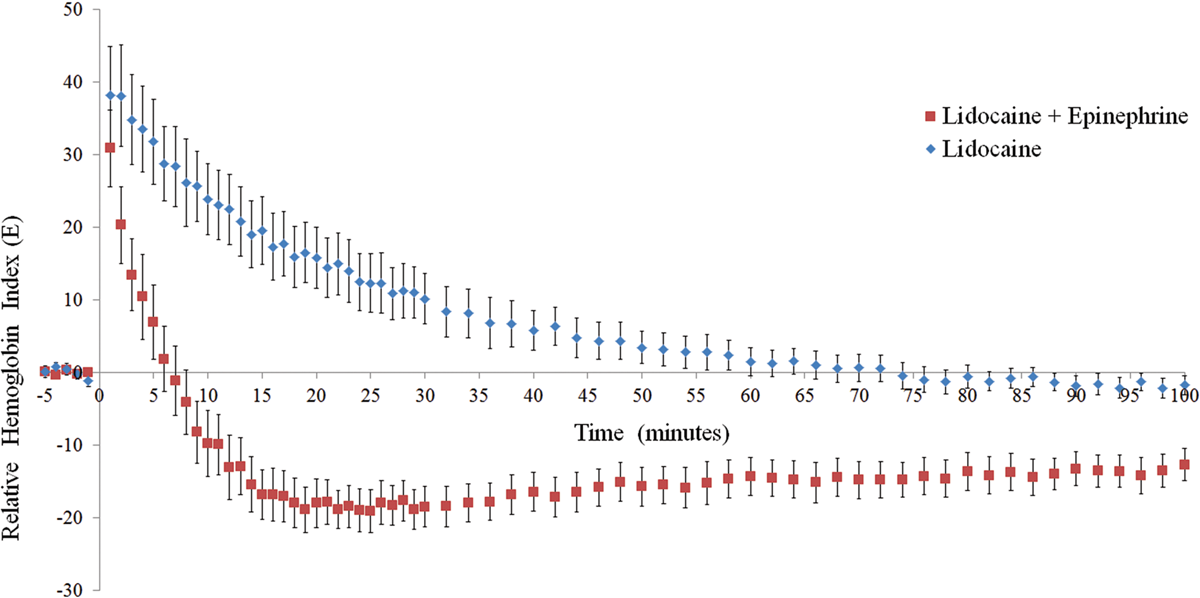
\includegraphics[width=1.0\textwidth]{figures/p2-mckee_fig.png}
	\caption[Sample time course of lidocaine and epinephrine]{\label{fig:p2-mckee_fig} Mean relative hemoglobin index (unitless) (y axis) versus time (in minutes) (x axis). Time = 0 is the injection of plain lidocaine (blue) and lidocaine plus epinephrine (red). Time < 0 represents baseline measurements. Error bars = SEM. The lowest point on the lidocaine plus epinephrine curve was -19.1, occurring at 25 minutes.}
\end{figure}

\section{Discussion}
This study revealed that the time when the lowest cutaneous hemoglobin concentration was obtained after injection of 1\% lidocaine with 1:100,000 epinephrine in the human arm was 25.9 minutes. This is considerably longer than the frequently quoted 7 to 10 minutes for maximal cutaneous vasoconstriction.\cite{Larrabee1987}

Several studies have used laser Doppler flowmetry in humans to correlate epinephrine concentration with arterial blood flow.\cite{Dunlevy1996,OMalley1995} No studies to date have used tissue reflectance spectroscopy to characterize the actual quantity of blood in soft tissue injected with lidocaine with epinephrine over time. This technique provides a more direct estimate of potential intraoperative bleeding, as opposed to measuring arterial blood flow alone.

Hemoglobin has a distinct spectral response and well-described absorption properties. Tissue reflectance spectroscopy is a validated reproducible technique for measuring oxygenated and deoxygenated hemoglobin concentrations in soft tissue at a depth of up to 1 cm.\cite{Dawson1980,Wilson2008} A widely used application of tissue spectroscopy in medicine is pulse oximetry. A pulse oximeter is specifically calibrated to distinguish the concentration of oxygenated hemoglobin in an arterial pulse from the soft tissue's total background hemoglobin concentration. In the present study, we were solely interested in background total hemoglobin. Tissue reflectance spectroscopy has been recently tested in plastic surgery for several novel purposes, including continuous noninvasive monitoring of tissue perfusion in free flaps, where changes in oxygenated hemoglobin concentration have been used to guide early reoperation in failing flaps.\cite{Najefi2010,Stelle2011} Spectroscopy is more reproducible, sensitive, and objective than color judgments made by the human eye when measuring degrees of paleness or erythema. In this study, spectral responses were found to be a reliable method used to distinguish the epinephrine and control groups. Mean relative hemoglobin index values at every time point after post injection minute 1 were significantly different between groups. The authors observed a correlation between spectroscopy measurements (relative hemoglobin index) and subjective visual observations (relative skin redness and whiteness) over time; however, this correlation was not quantified.

For each group, there was an immediate transient increase in hemoglobin index shown by spectroscopy that was statistically significant at 1 minute compared with baseline, using an unpaired two-tailed t test (p < 0.01). This immediate increase in hemoglobin is likely caused by local histamine release by mast cells because of tissue trauma from the injection and by the chemical sympathectomy effect of lidocaine, resulting in immediate vasodilation. In the plain lidocaine group, the hyperemia effect lasted up to 80 minutes on average. In the epinephrine group, hemoglobin concentration returned to baseline at roughly 7 minutes after injection, and continued to decrease until a new equilibrium was reached at roughly 25 minutes, with a hemoglobin concentration less than the baseline concentration. When using lidocaine, epinephrine should be added whenever possible to decrease bleeding during surgery.\cite{Higgins,Lalonde2011}

Epinephrine's vasoconstriction effect is complex, and vasoconstriction intensity differs depending on vessel type: arteries, arterioles, precapillary sphincters, capillaries, venules, and veins.\cite{Lee1050} Although epinephrine's maximal effect on arterial vasoconstriction may occur at 7 to 10 minutes, it takes considerably longer for a new local equilibrium to be obtained with regard to hemoglobin quantity.

If optimal visualization is desired, the ideal time for the surgeon to begin the incision should be the time when local hemoglobin concentration is lowest. Waiting 25 minutes after injection of local anesthetic with epinephrine before making an incision will result in less intraoperative bleeding. Plastic surgeons already using this concept may inject local anesthetic; leave the injected patient temporarily, to perform other tasks such as injecting other patients; and later return after roughly 25 minutes, to begin the procedure on the first patient.\cite{Gibson1990}

One limitation of this study was that there was no surgery performed on volunteers. Ideally, two standard bilateral incisions during a surgical procedure could be made at both 7 and 25 minutes after lidocaine plus epinephrine injection to see whether there was any difference in volume of blood loss between sites. Future studies could use spectroscopy to measure hemoglobin concentration in the head and neck or in the hand, as epinephrine likely has slightly different effects, depending on location.